\documentclass[12pt]{article}

\usepackage[a4paper,margin=1in]{geometry}
\usepackage{amsmath,amssymb}
\usepackage{tikz}
\usepackage{algorithm}
\usepackage{algpseudocode}

\usetikzlibrary{arrows.meta,positioning}

\title{Tromino Tiling: Mathematical Induction and Recursion}
\author{}
\date{}

\begin{document}

\maketitle

\section{Tiling a Deficient Chessboard with Trominoes}

A particularly elegant application of mathematical induction arises in a
tiling problem. A \emph{tromino} is a tile made from three unit squares.
We shall use an L-shaped tromino, as shown in Figure~\ref{fig:tromino}.
Rotations and reflections of the tile are also allowed.

\begin{figure}[ht]
\centering
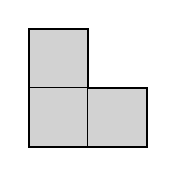
\begin{tikzpicture}[scale=0.75]

    \fill[gray!35] (0,0) rectangle (1,1);
    \fill[gray!35] (1,0) rectangle (2,1);
    \fill[gray!35] (0,1) rectangle (1,2);

    \draw[thick] (0,0) -- (2,0) -- (2,1) --
                 (1,1) -- (1,2) -- (0,2) -- cycle;

    \draw (1,0) -- (1,1);
    \draw (0,1) -- (1,1);

\end{tikzpicture}
\caption{An L-shaped tromino consisting of three unit squares.}
\label{fig:tromino}
\end{figure}


\subsection{The Tromino Tiling Problem}

Suppose one square is removed from a $2^n\times2^n$ chessboard,
where $n\geq1$. Can the remaining board always be tiled completely
using L-shaped trominoes, irrespective of which square is removed?

The answer is yes.

Let $P(n)$ denote the statement
\[
P(n):\qquad
\text{Every $2^n\times2^n$ board with one square removed
can be tiled with L-shaped trominoes.}
\]

We shall prove $P(n)$ by mathematical induction.


\subsection{Proof by Mathematical Induction}

\paragraph{Base case.}

For $n=1$, the board has size
\[
        2^1\times2^1=2\times2.
\]
It therefore consists of four unit squares. If any one square is
removed, the remaining three squares form exactly one L-shaped
tromino. Hence $P(1)$ is true.


\paragraph{Induction hypothesis.}

Suppose that $P(n)$ is true for some $n\geq1$. Thus we assume that
\emph{any} $2^n\times2^n$ board with one square removed can be tiled
completely using L-shaped trominoes.


\paragraph{Inductive step.}

We must show that $P(n+1)$ is true. Consider a
\[
        2^{n+1}\times2^{n+1}
\]
board from which one arbitrary square has been removed.

Divide the board into four equal quadrants. Each quadrant is a
$2^n\times2^n$ board. The missing square must lie in exactly one of
these four quadrants.

Without loss of generality, suppose that it lies in the top-left
quadrant, as illustrated in Figure~\ref{fig:tromino-induction}.

\begin{figure}[ht]
\centering

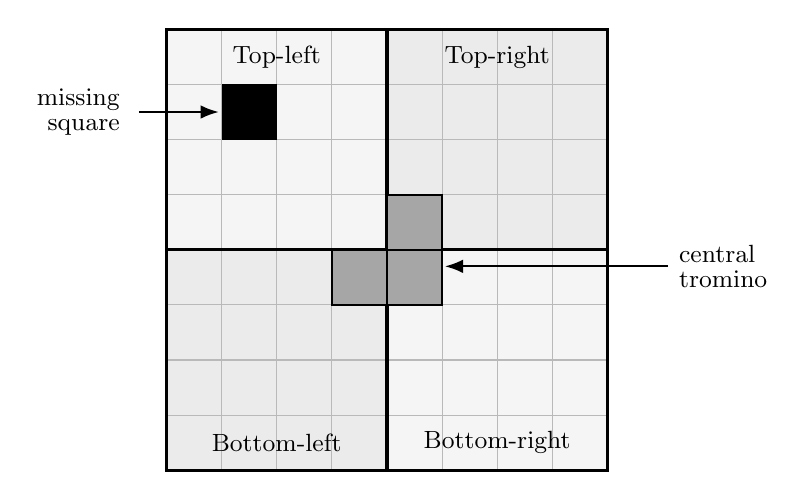
\begin{tikzpicture}[scale=0.70]

% An 8 x 8 board is used to illustrate the general construction.

% Shade the four quadrants lightly
\fill[gray!8]  (0,4) rectangle (4,8);
\fill[gray!16] (4,4) rectangle (8,8);
\fill[gray!16] (0,0) rectangle (4,4);
\fill[gray!8]  (4,0) rectangle (8,4);

% Grid
\draw[step=1,gray!55,thin] (0,0) grid (8,8);

% Outer boundary
\draw[very thick] (0,0) rectangle (8,8);

% Quadrant boundaries
\draw[very thick] (4,0) -- (4,8);
\draw[very thick] (0,4) -- (8,4);

% Original missing square in top-left quadrant
\fill[black] (1,6) rectangle (2,7);

% Central tromino:
% one square in top-right
\fill[gray!70] (4,4) rectangle (5,5);

% one square in bottom-left
\fill[gray!70] (3,3) rectangle (4,4);

% one square in bottom-right
\fill[gray!70] (4,3) rectangle (5,4);

% Borders of central tromino squares
\draw[thick] (4,4) rectangle (5,5);
\draw[thick] (3,3) rectangle (4,4);
\draw[thick] (4,3) rectangle (5,4);

% Quadrant labels
\node at (2,7.5) {\small Top-left};
\node at (6,7.5) {\small Top-right};
\node at (2,0.5) {\small Bottom-left};
\node at (6,0.5) {\small Bottom-right};

% Missing-square annotation
\draw[-{Latex},thick] (-0.5,6.5) -- (0.95,6.5);
\node[align=right] at (-1.6,6.5)
    {\small missing\\[-1mm]\small square};

% Central tromino annotation
\draw[-{Latex},thick] (9.1,3.7) -- (5.05,3.7);
\node[align=left] at (10.1,3.7)
    {\small central\\[-1mm]\small tromino};

\end{tikzpicture}

\caption{The $2^{n+1}\times2^{n+1}$ board is divided into four
$2^n\times2^n$ quadrants. The original missing square is shown in
black in the top-left quadrant. The shaded central L-shaped tromino
occupies one square in each of the other three quadrants.}
\label{fig:tromino-induction}
\end{figure}


Now comes the crucial observation. The top-left quadrant already has
one square missing. Place a single L-shaped tromino at the centre of
the board so that it occupies one central square in \emph{each of the
other three quadrants}.

After placing this central tromino:

\begin{enumerate}
    \item the top-left quadrant has exactly one square missing---the
          square that was originally removed;
    \item the top-right quadrant has exactly one square unavailable---the
          square occupied by the central tromino;
    \item the bottom-left quadrant similarly has exactly one square
          unavailable; and
    \item the bottom-right quadrant also has exactly one square
          unavailable.
\end{enumerate}

Thus we have transformed the original problem into four smaller
problems of precisely the form covered by the induction hypothesis.
Each quadrant is a $2^n\times2^n$ board with one square missing.

By the induction hypothesis, each of the four quadrants can therefore
be tiled completely with L-shaped trominoes. Together with the one
tromino that we have already placed at the centre, these tilings cover
the entire $2^{n+1}\times2^{n+1}$ board except for the originally
removed square.

Hence
\[
        P(n)\Longrightarrow P(n+1).
\]

Since $P(1)$ is true, the Principle of Mathematical Induction gives
\[
\boxed{
\text{Every $2^n\times2^n$ board with one square removed can be
tiled completely with L-shaped trominoes.}
}
\]


\section{The Inductive Proof is a Recursive Algorithm}

The proof above does more than establish that a tiling exists. It
actually tells us \emph{how to construct one}. Hidden inside the
inductive proof is therefore a recursive algorithm.

Suppose we are given a $2^n\times2^n$ board and the position of its
one missing square. Let us call the procedure
\[
        \textsc{Tile}(B,n,x),
\]
where $B$ is the board and $x$ is its missing square.

The inductive proof suggests the following procedure.

\begin{enumerate}

\item If $n=1$, then $B$ is a $2\times2$ board. Since one square is
missing, place one L-shaped tromino on the remaining three squares.
The problem is solved.

\item Otherwise, divide $B$ into four equal
$2^{n-1}\times2^{n-1}$ quadrants.

\item Determine which quadrant contains the missing square $x$.

\item Place one L-shaped tromino at the centre of the board so that
it occupies one central square in each of the \emph{other three}
quadrants.

\item We now have four smaller boards, each with exactly one square
missing:
\begin{itemize}
    \item in one quadrant it is the original missing square $x$;
    \item in each of the other three quadrants it is the square
          occupied by the central tromino.
\end{itemize}

\item Apply exactly the same procedure recursively to each of these
four smaller boards.

\end{enumerate}

Thus a problem on a $2^n\times2^n$ board is reduced to four problems
on boards of size
\[
        2^{n-1}\times2^{n-1}.
\]
Each of these is again reduced to four still smaller problems, and so
on, until we reach $2\times2$ boards.


\subsection{The Recursive Algorithm}

The construction can be written as the following algorithm.

\begin{algorithm}[ht]
\caption{Recursive algorithm for tiling a deficient
$2^n\times2^n$ board}
\label{algo:tromino}
\begin{algorithmic}[1]

\Procedure{Tile}{$B,n,x$}

\If{$n=1$}
    \State Place one L-shaped tromino on the three squares of $B$
           other than $x$
    \State \Return
\EndIf

\State Divide $B$ into four equal quadrants
       $B_1,B_2,B_3,B_4$

\State Let $B_i$ be the quadrant containing the missing square $x$

\State Place an L-shaped tromino at the centre so that it occupies
       one central square in each quadrant $B_j$, $j\neq i$

\For{$j=1,2,3,4$}
    \If{$j=i$}
        \State $x_j \gets x$
    \Else
        \State $x_j \gets$ the central square of $B_j$
               covered by the newly placed tromino
    \EndIf
    \State \Call{Tile}{$B_j,n-1,x_j$}
\EndFor

\EndProcedure

\end{algorithmic}
\end{algorithm}


\subsection{The Recursion Tree}

The recursive structure can be represented as a tree. A problem on a
$2^n\times2^n$ board generates four problems on
$2^{n-1}\times2^{n-1}$ boards. Each of those generates four still
smaller problems.

\begin{figure}[ht]
\centering

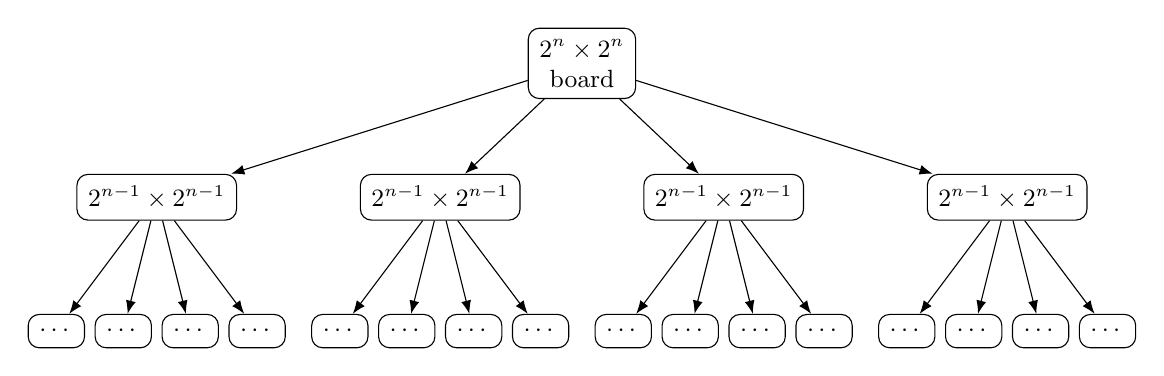
\begin{tikzpicture}[
    level distance=1.7cm,
    level 1/.style={sibling distance=3.6cm},
    level 2/.style={sibling distance=0.85cm},
    every node/.style={
        draw,
        rounded corners,
        align=center,
        font=\small,
        inner sep=4pt
    },
    edge from parent/.style={draw,-{Latex}}
]

\node {$2^n\times2^n$\\board}
    child {node {$2^{n-1}\times2^{n-1}$}
        child {node {$\cdots$}}
        child {node {$\cdots$}}
        child {node {$\cdots$}}
        child {node {$\cdots$}}
    }
    child {node {$2^{n-1}\times2^{n-1}$}
        child {node {$\cdots$}}
        child {node {$\cdots$}}
        child {node {$\cdots$}}
        child {node {$\cdots$}}
    }
    child {node {$2^{n-1}\times2^{n-1}$}
        child {node {$\cdots$}}
        child {node {$\cdots$}}
        child {node {$\cdots$}}
        child {node {$\cdots$}}
    }
    child {node {$2^{n-1}\times2^{n-1}$}
        child {node {$\cdots$}}
        child {node {$\cdots$}}
        child {node {$\cdots$}}
        child {node {$\cdots$}}
    };

\end{tikzpicture}

\caption{The recursive structure of the tromino tiling algorithm.
Each problem is reduced to four problems with half the side length.
The recursion eventually reaches $2\times2$ boards.}
\label{fig:tromino-recursion}
\end{figure}


\section{Induction and Recursion}

Notice how closely the recursive algorithm follows the inductive proof.
The two parts correspond almost exactly.

\begin{center}
\renewcommand{\arraystretch}{1.5}
\begin{tabular}{|p{0.40\textwidth}|p{0.48\textwidth}|}
\hline
\textbf{Inductive proof} & \textbf{Recursive algorithm}\\
\hline

Establish the base case $P(1)$.
&
Directly tile a $2\times2$ board.
\\
\hline

Assume that every smaller $2^{n-1}\times2^{n-1}$ deficient board can
be tiled.
&
Call \textsc{Tile} recursively on the four smaller deficient boards.
\\
\hline

Use the induction hypothesis to prove the result for the larger
$2^n\times2^n$ board.
&
Use the four recursively constructed tilings, together with the
central tromino, to construct the tiling of the larger board.
\\
\hline
\end{tabular}
\end{center}

Mathematical induction and recursion are therefore closely related.
Induction is a method for \emph{proving} that a construction works for
problems of every size, whereas recursion is a method for
\emph{carrying out} the construction by solving smaller instances of
the same problem.

There is an important difference in viewpoint:
\[
\begin{array}{ccl}
\text{Induction} &:&
\text{If I can solve the smaller problem, I can prove that the
larger problem can be solved;}\\[1mm]
\text{Recursion} &:&
\text{To solve the larger problem, actually solve the smaller
problems using the same procedure.}
\end{array}
\]

The tromino problem makes this connection particularly visible.


\section{A Recurrence for the Number of Trominoes}

The recursive construction also allows us to count how many trominoes
are used.

Let $T(n)$ denote the number of trominoes required to tile a
$2^n\times2^n$ board with one square removed.

For the base case,
\[
        T(1)=1.
\]

For $n>1$, the algorithm first places one tromino at the centre. It
then recursively tiles four boards of size
$2^{n-1}\times2^{n-1}$. Therefore
\[
        \boxed{T(n)=4T(n-1)+1.}
\]

This is called a \emph{recurrence relation}: it defines the value of
$T(n)$ in terms of the value of the same function for a smaller
argument.

We can also determine $T(n)$ simply by counting squares. A
$2^n\times2^n$ board contains
\[
        2^n\,2^n=4^n
\]
unit squares. One square has been removed, so the number of squares
that must be covered is
\[
        4^n-1.
\]

Since every tromino covers exactly three squares, the number of
trominoes must be
\[
        T(n)=\frac{4^n-1}{3}.
\]

This agrees with the recurrence. Indeed, suppose
\[
        T(n-1)=\frac{4^{n-1}-1}{3}.
\]
Then
\[
\begin{aligned}
T(n)
    &=4T(n-1)+1\\
    &=4\left(\frac{4^{n-1}-1}{3}\right)+1\\
    &=\frac{4^n-4}{3}+1\\
    &=\frac{4^n-1}{3}.
\end{aligned}
\]

Thus
\[
        \boxed{T(n)=\frac{4^n-1}{3}}.
\]

For example, an $8\times8$ board corresponds to $n=3$. It contains
$64$ squares, of which one is missing. Hence the tiling requires
\[
        T(3)=\frac{4^3-1}{3}
             =\frac{63}{3}
             =21
\]
trominoes.


\section{Proof, Algorithm, and Recurrence}

The tromino problem illustrates several ideas that recur throughout
mathematics and computer science.

Starting with a single problem, we have obtained the chain
\[
\boxed{
\text{inductive proof}
\;\longrightarrow\;
\text{constructive proof}
\;\longrightarrow\;
\text{recursive algorithm}
\;\longrightarrow\;
\text{recurrence relation}.
}
\]

The inductive proof tells us \emph{why} a tiling must exist. The proof
is constructive because it tells us how to build such a tiling. That
construction becomes a recursive algorithm because it repeatedly
reduces the problem to smaller instances of itself. Finally, examining
the recursive algorithm naturally produces a recurrence relation.

This is an important connection between mathematical reasoning and
computation: a proof may not merely tell us that a solution exists;
sometimes it also contains an algorithm for finding one.

\end{document}
